\documentclass[12pt]{article}

\usepackage[spanish]{babel}
\usepackage{hyperref}
\usepackage{graphicx}
\usepackage{listings}
\usepackage{color}
\usepackage{multicol}
\usepackage{amssymb}
\spanishdecimal{.}
\usepackage{enumitem}
\usepackage{here}
\usepackage{dsfont}
\usepackage{amsmath}


%% Título
\title{Matemáticas para las Ciencias Aplicadas I}
\title{
	Segunda Lista de Problemas \\
	\vspace{1ex}
	\large Matemáticas para las Ciencias Aplicadas I \\
	Facultad de Ciencias, UNAM}

%% Fecha
\date{\today}

%% Autor
\author{Flores Morán Julieta Melina \\ Zarco Romero José Antonio}

%% Se marca el inicio del documento.
\begin{document}

%%
%%Comando para crear el título.
\maketitle
\subsection*{\centering \textbf{ \LARGE Primera Parte}}
%1
\section{Ejercicio 3}
Flores Morán Julieta Melina \\
\begin{enumerate}[label=(\alph*)]
\item Aproximar el valor del límite
\[
\lim_{x \to 0}\frac{3^x-2^x}{x}
\]
hasta tres decimales mediante la construcción de una tabla de valores apropiada.\\
\begin{center}
\begin{tabular}{|c|c|c|}
\hline
\(x\) & \(\frac{3^x-2^x}{x}\) & \(\frac{3^x-2^x}{x}\) \\[0.8ex] 
\hline
0.1 & \(\frac{3^{0.1}-2^{0.1}}{0.1}\) & $0.443$\\ [0.8ex] 
0.01 & \(\frac{3^{0.01}-2^{0.01}}{0.01}\) & $0.409$ \\[0.8ex] 
0.001 & \(\frac{3^{0.001}-2^{0.001}}{0.001}\) & $0.405$ \\[0.8ex] 
0.0001 & \(\frac{3^{0.0001}-2^{0.0001}}{0.0001}\)  & $0.405$ \\[0.8ex] 
0.00001 & \(\frac{3^{0.00001}-2^{0.00001}}{0.00001}\)& $0.405$ \\[0.8ex] 
0.000001 & \(\frac{3^{0.000001}-2^{0.000001}}{0.000001}\)& $0.405$ \\[0.8ex] 
\hline
\end{tabular}
\end{center}
Con esta tabla podemos observar que el valor de $\lim_{x \to 0}\frac{3^x-2^x}{x}$ se acerca a 0.405 conforme x tiende a 0.

\item Confirme su aproximación utilizando evidencia gráfica.
\begin{figure}[h!]
\centering
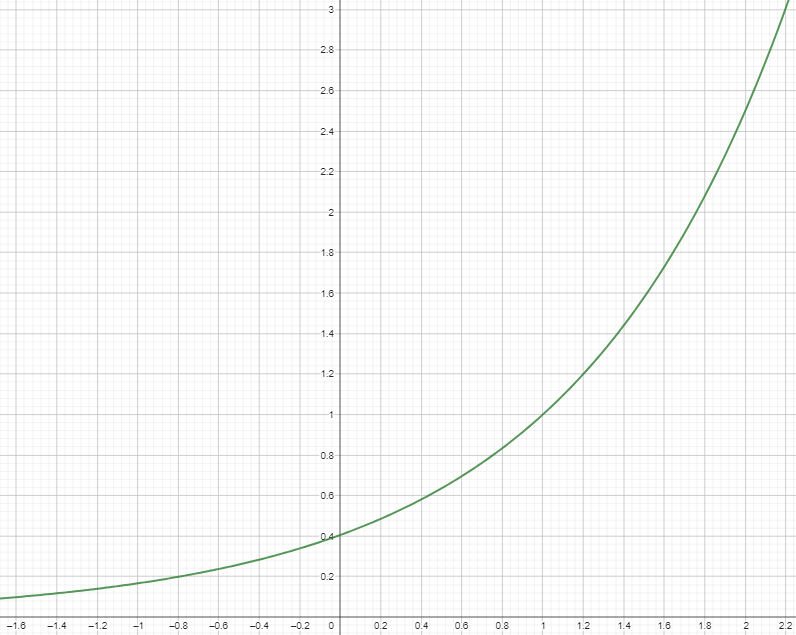
\includegraphics[width=1\textwidth]{../img/img_Lista2/ej3.png}
\end{figure}
\end{enumerate}
\[
\therefore \lim_{x \to 0}\frac{3^x-2^x}{x} \approx 0.405
\]
%2
\section{Ejercicio 9}
Zarco Romero José Antonio\\
\[
\lim_{x \to +\infty}\frac{(2x-1)^5}{(3x^2+2x-7)(x^3-9x)}
\]
Para resolver este límite primero reescribiremos la expresión algebraica.
\[
\frac{(2x-1)^5}{(3x^2+2x-7)(x^3-9x)} = \frac{32x^{5}-80x^{4}+80x^{3}-40x^{2}+10x-1}{3x^{5}+2x^{4}-34x^{3}-18x^{2}+63x} \cdot \frac{\frac{1}{x^{5}}}{\frac{1}{x^{5}}}
\]
\[
\frac{ \frac{32x^{5}-80x^{4}+80x^{3}-40x^{2}+10x-1 }{x^{5}}}{ \frac{3x^{5}+2x^{4}-34x^{3}-18x^{2}+63x}{x^{5}}} = \frac{  \frac{32x^{5}}{x^{5}} - \frac{80x^{4}}{x^{5}} + \frac{80x^{3}}{x^{5}} - \frac{40x^{2}}{x^{5}} + \frac{10x}{x^{5}}- \frac{1}{x^{5}} }{
\frac{3x^{5}}{x^{5}} + \frac{2x^{4}}{x^{5}} - \frac{34x^{3}}{x^{5}} - \frac{18x^{2}}{x^{5}} + \frac{63x}{x^{5}}}
\]
\[ =
\frac
{  
	32 - \frac{80}{x} + \frac{80}{x^{2}} - \frac{40}{x^{3}} + \frac{10}{x^{4}}- \frac{1}{x^{5}} 
}
{
	3 + \frac{2}{x} - \frac{34x}{x^{2}} - \frac{18}{x^{3}} + \frac{63}{x^{4}}
}
\]
Ahora será más fácil calcular el límite de la función, considerando que un número divido entre un número muy grande tiende a 0.
\[
\lim_{x \to +\infty}
\frac{  
	32 - \frac{80}{x} + \frac{80}{x^{2}} - \frac{40}{x^{3}} + \frac{10}{x^{4}}- \frac{1}{x^{5}} 
}{
	3 + \frac{2}{x} - \frac{34x}{x^{2}} - \frac{18}{x^{3}} + \frac{63}{x^{4}}
}
= \frac{\lim_{x \to +\infty}
	32 - \frac{80}{x} + \frac{80}{x^{2}} - \frac{40}{x^{3}} + \frac{10}{x^{4}}- \frac{1}{x^{5}} 
}{\lim_{x \to +\infty}
	3 + \frac{2}{x} - \frac{34x}{x^{2}} - \frac{18}{x^{3}} + \frac{63}{x^{4}}}
\]
\[=\frac{
	\lim_{x \to +\infty}32 - 
	\lim_{x \to +\infty}\frac{80}{x} + 
	\lim_{x \to +\infty}\frac{80}{x^{2}} - 
	\lim_{x \to +\infty}\frac{40}{x^{3}} + 
	\lim_{x \to +\infty}\frac{10}{x^{4}}- 
	\lim_{x \to +\infty}\frac{1}{x^{5}} 
}{
	\lim_{x \to +\infty}3 + 
	\lim_{x \to +\infty}\frac{2}{x} - 
	\lim_{x \to +\infty}\frac{34x}{x^{2}} - 
	\lim_{x \to +\infty}\frac{18}{x^{3}} + 
	\lim_{x \to +\infty}\frac{63}{x^{4}}}
\]
\[
= \frac{32 - 0 + 0 - 0 + 0- 0 }{3 + 0- 0-0+ 0}
= \frac{32}{3}
\]
\[
\therefore \lim_{x \to +\infty}\frac{(2x-1)^5}{(3x^2+2x-7)(x^3-9x)} = \frac{32}{3}
\]
%3
\section{Ejercicio 18}
Flores Morán Julieta Melina \\
\[
\lim_{\theta \to 0^+} \ln (\sin 2\theta) - \ln (\tan \theta)
\]
Primero reescribiremos la expresión
\[
 \ln (\sin 2\theta) - \ln (\tan \theta) = \ln ( \frac{\sin 2\theta}{\tan \theta} ) 
\]
Considerando la fórmula para el seno de la suma de ángulos $ \sin (\alpha + \beta) = \sin \alpha \cdot \cos \beta + \cos \alpha \cdot \sin \beta $, donde en este caso $\alpha = \beta = \theta$ se puede calcular que $\sin 2\theta = sin \theta \cdot \cos \theta  + \cos \theta  \cdot \sin \theta   = 2 \cdot \cos \theta  \cdot \sin \theta $ \\
Entonces 
\[
 \frac{\sin 2\theta}{\tan \theta} = \frac{ 2 \cdot \cos \theta  \cdot \sin \theta}{\frac{\sin \theta}{\cos \theta}} = \frac{2 \cdot \cos \theta  \cdot \sin \theta \cdot \cos \theta}{sin \theta} = \frac{2 \cdot \sin \theta}{\sin \theta} \cdot [\cos \theta]^{2} = 2 \cdot [\cos \theta]^{2}
\]
\[
\therefore \ln ( \frac{ \sin 2 \theta }{ \tan \theta} ) = ln ( 2 \cdot [\cos \theta]^{2} )
\]
Ahora será más fácil calcular el límite de esta expresión
\[
\lim_{\theta \to 0^+} \ln (\sin 2\theta) - \ln (\tan \theta) = \lim_{\theta \to 0^+}  ln ( 2 \cdot [\cos \theta]^{2} ) =  ln ( \lim_{\theta \to 0^+} ( 2 \cdot [\cos \theta]^{2} )) 
\]
\[
= ln (  2 \cdot [\cos 0]^{2}) =ln (  2 \cdot 1^{2})  = ln (2) 
\]
\[
\therefore \lim_{\theta \to 0^+} \ln (\sin 2\theta) - \ln (\tan \theta) =  ln (2) 
\]
%4
\section{Ejercicio 20}
Zarco Romero José Antonio\\
\[
\lim_{x \to + \infty} (1+\frac{a}{x})^{bx} ~ ~ ~,~ ~ a,b>0
\]
Supongamos que $t=\frac{a}{x}$ y, despejando $x=\frac{a}{t}$. Por lo anterior, se tiene que si $x$ tiende a $+ \infty$, entonces $t$ tiende a $0$. Por lo tanto, la fórmula original queda reescrita como:
\[
\lim_{t \to 0} (1+t)^{b \cdot \frac{a}{t}}
= \lim_{t \to 0} (1+t)^{\frac{1}{t} \cdot a \cdot b}
= [\lim_{t \to 0} (1+t)^{\frac{1}{t}}]^{a \cdot b}
= e^{a \cdot b}
\]
\[
\therefore \lim_{x \to + \infty} (1+\frac{a}{x})^{bx}
= e^{a \cdot b}
 ~ ~ ~ ~\text{donde}~ ~ a,b>0
\]

%5
\section{Ejercicio 31}
Zarco Romero José Antonio\\
\\
Encuentre valores de $x$, si los hay, en los que la función dada no sea continua.
\begin{enumerate}[label=(\alph*)]
\item \[ f(x)=\frac{x}{x^2-1} \]
Sabemos que las funciones $y=x$ y $y=x^2-1$ son funciones polinomiales. De modo que son continuas en todo su dominio (para toda $x$); es decir, son continuas sobre $\mathbb R=(-\infty,\infty)$. Ahora, la función $f(x)=\frac{x}{x^2-1}$ es racional, así que es continua siempre que está definida; es decir, en su dominio que es $\{ x ~|~ (x^2-1) \neq 0 \}$. Si $x^2-1=0$, entonces:
\[
x^2-1=0
\]
\[
x^2=1
\]
\[
x=\sqrt{1}
\]
\[
x_0=1 \text{ , } x_1=-1
\]
$\therefore$ La función $f(x)=\frac{x}{x^2-1}$ no es continua en los valores de $x_0=1 \text{ y } x_1=-1$.

\item \[ f(x)= | x^3-2x^2 | \]
\begin{enumerate}
	\item[1)] La función dada es polinomial, por lo que está definida para toda $x$.
	\item[2)] Calculando los límites laterales cuando $x$ se acerca a un punto $a$.
	\begin{itemize}
		\item Límite derecho en $a$:
		\[ 
		\lim_{x \to a^+}f(x) = \lim_{x \to a^+}| x^3-2x^2 | =\lim_{x \to a^+}| a^3-2a^2 |
		\]
		\item Límite izquierdo en $a$:
		\[ 
		\lim_{x \to a^-}f(x) = \lim_{x \to a^-}| x^3-2x^2 | =\lim_{x \to a^-}| a^3-2a^2 |
		\]
	\end{itemize}
	Dado que los límites son iguales, entonces el límite existe para cualquier $a$.
	\item[3)] Por el punto anterior, el valor del límite cuando $x$ tiende a $a$ es igual al valor de la función en $a$.
\end{enumerate}
$\therefore$ La función $f(x)= |x^3-2x^2 |$ es continua para toda $x$.

\item \[ f(x)=\frac{x+3}{~|x^2+3x|~} \]
La función es racional, así que es continua siempre que está definida; es decir, en su dominio que es $\{ x ~|~ ~|x^2+3x|\neq 0 \}$. Si $|x^2+3x|=0$, entonces:
\[
|x^2+3x|=0
\]
\[
x^2+3x=0
\]
\[
x(x+3)=0
\]
\[
x_0=0 \text{ , } x_1=-3
\]
$\therefore$ La función $f(x)=\frac{x+3}{~|x^2+3x|~}$ no es continua en los valores de $x_0=0 \text{ y } x_1=-3$.
\end{enumerate}

%6
\section{Ejercicio 36}
Flores Morán Julieta Melina \\
\\
Supongamos que $f$ es continua en el intervalo $[0, 1]$, que $f(0) = 2$ y que $f$ no tiene ceros en el intervalo. Demuestre que $f(x) > 0$ para todo $x$ en $[0, 1]$.\\ 

Podemos utilizar el El Teorema del Valor Intermedio para demostrarlo. Este Teorema enuncia para este caso que, sea N un valor entre f(0) y f (1), cumple que $f(0)<N<f(1)$ ó $f(1)<N<f(0)$ y existe un $c \in (0, 1)$ tal que $f(c) = N$.\\
Lo que queremos demostrar es que $N>0$ para cualquier $c \in (0, 1)$. \\
Considerando que $f(0) = 2 $ podemos considerar que $2<N<f(1)$ ó $f(1)<N<2$  \\
En el primer caso donde la función es creciente, $2<N$ asegura que $N>0$ \\
En el segundo caso, tenemos que considerar que $f(1)>0$ ya que de lo contrario, según el Teorema del Valor Intermedio $f(c)$ tendría que ser $0$ para alguna $c \in (0, 1)$ ya que 0 es un valor intermedio entre $f(0) = 2$ y cualquier número negativo. Ya que se garantiza que no hay ceros en el intervalo [0,1], $f(1)$ debe ser positivo, y por tanto en la desigualdad  $f(1)<N<f(0)$ si $f(1)<N$, entonces N es número positivo y por tanto $N>0$
\subsection*{\centering \textbf{ \LARGE Segunda Parte}}
%% 5, 10, 20, 36 y 40

%% 1
\section{Ejercicio 5} Zarco Romero José Antonio \\

Utilice una aproximación cuadrática local apropiada para aproximar $\tan 61^{\circ}$ y compare el resultado con el producido directamente por su utilidad de cálculo. \\

A fin de encontrar una fórmula para la aproximación cuadrática local de una función $f$ acerca de $x=x_0$. Esta aproximación tiene la forma:
\[p_2(x)=f(x_0)+f'(x_0)(x-x_0)+\frac{f''(x_0)}{2!}(x-x_0)^2\]
Dado que $61^{\circ} = \frac{\pi}{3} + \frac{\pi}{180} rad$. Entonces, sea $f(x_0)=\tan x_0$ y $x_0=\frac{\pi}{3}$; de este modo:
\begin{center}
\begin{tabular}{r l}
$f(x_0)=\tan x_0$ & $f(\frac{\pi}{3})=\tan \frac{\pi}{3}=\sqrt 3 rad$ \\
$f'(x_0)=(\sec x_0)^2$ & $f'(\frac{\pi}{3})=(\sec \frac{\pi}{3})^2=4 rad$ \\
$f''(x_0)=2 (\sec x_0)^2 \tan x_0$ & $f''(\frac{\pi}{3})=2 (\sec \frac{\pi}{3})^2 \tan \frac{\pi}{3}=8\sqrt 3 rad$ \\
\end{tabular}
\end{center}
Sustituyendo los valores, tenemos que:
\[
p_2(x)=\sqrt 3 + 4(x-\frac{\pi}{3}) + \frac{8 \sqrt 3}{2 \cdot 1}(x-\frac{\pi}{3})^2
=\sqrt 3 + 4(x-\frac{\pi}{3}) + 4 \sqrt 3(x-\frac{\pi}{3})^2
\]
Ya que $x=61^{\circ}=\frac{\pi}{3} + \frac{\pi}{180}rad$
\[
p_2(\frac{\pi}{3} + \frac{\pi}{180}rad)
=\sqrt 3 + 4[(\frac{\pi}{3} + \frac{\pi}{180}rad)-\frac{\pi}{3}] + 4 \sqrt 3[(\frac{\pi}{3} + \frac{\pi}{180}rad)-\frac{\pi}{3}]^2
\]
\[
=\sqrt 3 + 4(\frac{\pi}{180}rad) + 4 \sqrt 3(\frac{\pi}{180}rad)^2
= \sqrt 3 + \frac{\pi}{45}rad + 4 \sqrt 3(\frac{\pi}{180}rad)^2
\]
\[\therefore p_2(61^{\circ}) \approx 1.803974\]
El valor de la aproximación cuadrática local fue de $1.803974$, mientras que el producido directamente por la calculadora fue de $1.804047$.

%% 2
\section{Ejercicio 10} Zarco Romero José Antonio \\

Encuentre los polinomios de Maclaurin de orden $n = 0, 1, 2, 3, 4$, y luego encuentre los polinomios de Maclaurin enésimos para la función en notación sigma.
\[\sin \pi x\]

Sea $f(x)=\sin \pi x$; de este modo:
\begin{center}
  \begin{tabular}{r l}
    $f(x)=\sin (\pi x)$ & $f(0)=0$ \\
    $f'(x)=\pi \cos (\pi x)$ & $f'(0)=\pi$ \\
    $f''(x)= - \pi ^2 \sin (\pi x)$ & $f''(0)=0$ \\
    $f'''(x)= - \pi ^3 \cos (\pi x)$ & $f'''(0)=-\pi ^3$ \\
    $f^{(4)}(x)= \pi ^4 \sin (\pi x)$ & $f^{(4)}(0)=0$ \\
  \end{tabular}
\end{center}
Dado que el patrón $0, \pi ^k, 0, -\pi ^k$ se repetirá a medida que evaluemos derivadas sucesivas en 0; ya que $f^{(k)}(x)=0$ cuando $k$ es par y, cuando $k$ es impar el resultado de $f^{(k)}(x)$ alterna entre $\pi ^k$ y $-\pi ^k$.
Por lo tanto, los polinomios de Maclaurin de orden $n = 0, 1, 2, 3, 4$ para $\sin \pi x$ son:
\begin{center}
  \begin{tabular}{l}
    $p_0(x)=0$ \\
    $p_1(x)=0+\pi x=\pi x$ \\
    $p_2(x)=0+\pi x+0=\pi x$ \\
    $p_3(x)=0+\pi x+0+\frac{-\pi ^3}{3!}x^3=\pi x- \frac{\pi ^3}{3!}x^3=\pi - \frac{\pi ^3}{6}x^3$ \\
    $p_4(x)=0+\pi x+0+\frac{-\pi ^3}{3!}x^3+0=\pi x - \frac{\pi ^3}{3!}x^3+0=\pi - \frac{\pi ^3}{6}x^3$ \\
  \end{tabular}
\end{center}
Se obtiene el enésimo polinomio de Maclaurin para la función $\sin \pi x$ en notación sigma.
\[
p_n(x)=\sum_{k=0}^{n} \frac{(\pi)^k \cdot \sin(\frac{k \pi }{2})}{k!}(x)^k
\]

%% 3
\section{Ejercicio 20} Zarco Romero José Antonio \\

Encuentre los polinomios de Taylor de orden $n = 0, 1, 2, 3, 4$ alrededor de $x = x_0$ y luego encuentre el enésimo polinomio de Taylor para la función en notación sigma.
\[\frac{1}{x+2}\text{; }x_0=3\]

Sea $f(x_0)=\frac{1}{x_0+2}$ y $x_0=3$; de este modo:
\begin{center}
  \begin{tabular}{r l}
    $f(x_0)=\frac{1}{x_0+2}$ & $f(3)=\frac{1}{3+2}=\frac{1}{5}$\\
    $f'(x_0)=-\frac{1}{(x_0+2)^2}$ & $f'(3)=-\frac{1}{(3+2)^2}=-\frac{1}{5^2}=-\frac{1}{25}$\\
    $f''(x_0)=\frac{2}{(x_0+2)^3}$ & $f''(3)=\frac{2}{(3+2)^3}=\frac{2}{5^3}=\frac{2}{125}$\\
    $f'''(x_0)=-\frac{6}{(x_0+2)^4}$ & $f'''(3)=-\frac{6}{(3+2)^4}=-\frac{6}{5^4}=-\frac{6}{625}$ \\
    $f^{(4)}(x_0)=\frac{24}{(x_0+2)^5}$ & $f^{(4)}(3)=\frac{24}{(3+2)^5}=\frac{24}{5^5}=\frac{24}{3125}$ \\
    $\vdots$ & $\vdots$ \\
    $f^{(k)}(x_0)=\sum_{k=0}^{n} (-1)^k \frac{k!}{(x+2)^{k+1}}$ & $f^{(k)}(3)=\sum_{k=0}^{n} (-1)^k \frac{k!}{5^{k+1}}$ \\
  \end{tabular}
\end{center}
Por lo tanto, los polinomios de Taylor de orden $n = 0, 1, 2, 3, 4$ para $f(x)=\frac{1}{x+2}$ alrededor de $x_0 = 3$ son:
\begin{center}
  \begin{tabular}{l}
    $p_0(x)=\frac{1}{5}$ \\
    $p_1(x)=\frac{1}{5}+(-\frac{1}{25})x=\frac{1}{5}-\frac{1}{25}x$ \\
    $p_2(x)=\frac{1}{5}+(-\frac{1}{25})x+\frac{\frac{2}{125}}{2!}(x-3)^2=\frac{1}{5}-\frac{1}{25}x+\frac{1}{125}(x-3)^2$ \\
    $p_3(x)=\frac{1}{5}+(-\frac{1}{25})x+\frac{\frac{2}{125}}{2!}(x-3)^2+\frac{-\frac{6}{625}}{3!}(x-3)^3$ \\
    $=\frac{1}{5}-\frac{1}{25}x+\frac{1}{125}(x-3)^2-\frac{1}{625}(x-3)^3$ \\
    $p_4(x)=\frac{1}{5}+(-\frac{1}{25})x+\frac{\frac{2}{125}}{2!}(x-3)^2+\frac{-\frac{6}{625}}{3!}(x-3)^3+\frac{\frac{24}{3125}}{4!}(x-3)^4$ \\
    $=\frac{1}{5}-\frac{1}{25}x+\frac{1}{125}(x-3)^2-\frac{1}{625}(x-3)^3+\frac{1}{3125}(x-3)^4$ \\
  \end{tabular}
\end{center}
Por tanto, sustituyendo $f^{(k)}(x_0)=\sum_{k=0}^{n} (-1)^k \frac{k!}{(x+2)^{k+1}}$ en la fórmula
\[ \sum_{k=0}^{n} \frac{f^{(k)}(x_0)}{k!}(x-x_0)^k \]
Se obtiene el enésimo polinomio de Taylor para la función $\frac{1}{x+2} \text{; } x_0=3$ en notación sigma.
\[
p_n(x)=\sum_{k=0}^{n} \frac{(-1)^k}{5^{k+1}}(x-3)^k
\]

%% 4
\section{Ejercicio 36} Flores Morán Julieta Melina \\

Utilice el método del ejemplo 7 para aproximar la expresión dada a la precisión especificada. Verifique su respuesta con la producida directamente por su utilidad de cálculo.
\[\frac{1}{e}\text{; precisión de tres decimales}\]
Sabiendo que $ \frac{1}{e} = e^{-1} $, podemos usar el enésimo polinomio de Maclaurín de $e^{x}$ para aproximar $e^{-1}$ con una precisión de tres decimales considerando que la función exponencial $e^{x}$ tiene derivadas de cualquier orden para todos los números reales x.\\
El enésimo polinomio de Maclaurin para $e^x$ es:
\[
\sum_{k=0}^{n}\frac{x^{k}}{k!} = 1 + x + \frac{x^{2}}{2!}+ \cdots + \frac{x^{n}}{n!}
\]
Por la cual obtenemos para $x = -1$
\[
e^{-1} \approx \sum_{k=0}^{n}\frac{(-1)^{k}}{k!} = 1 - 1 + \frac{1}{2!}+ \cdots + \frac{(-1)^{n}}{n!}
\]
El problema consiste en determinar cuantos términos incluir en e polinomio de Maclaurin de $e^{-1}$ para alcanzar una precisión de tres decimales. Esto requiera que encontremos una $n$ para la cual el valor absoluto de el enésimo residuo en $x = -1$ cumpla
\[
\left| R_n (-1) \right| \leq 0.0005
\]
Para determinar $n$ usamos el el Teorema de Estimación del Residuo 
remplazando la inecuación del teorema 
\[
\left| R_n (x)  \right|  \leq \frac{M}{(n+1)!} \left| x-x_0  \right|^{n+1}
\]
Con $f(x) = e ^{x}$, $x = -1$, $x_0 = 0$ y el intervalo $[-1, 0]$ obtenemos
\[
\left| R_n (-1)  \right|  \leq \frac{M}{(n+1)!} \left| -1-0  \right|^{n+1}
\]
Donde M es una cota superior en el intervalo $f^{n+1}(x) = e^{x}$ para x en el intervalo $[-1, 0]$, esto es $\left|f^{n+1}(x)\right| \leq M$ para toda  x en el intervalo. $e^x$ es una función creciente, así que su máximo valor en el intervalo $[-1, 0]$ ocurre en $x=0$, es decir, $e^{x} \leq e^{0} =1$ en este intervalo. Entonces podemos considerar $M = 1$ para obtener:
\begin{eqnarray}
\left| R_n (-1)  \right| = \left| e^{-1}- p_n(-1)  \right|
&\leq & \frac{1}{(n+1)!} \left| -1\right|^{n+1} \nonumber
\\
&\leq & \frac{1}{(n+1)!} (1)^{n+1} \nonumber
\\
&\leq & \frac{1}{(n+1)!}  \nonumber
\end{eqnarray}
Con esta inecuación podemos alcanzar tres decimales de precisión encontrando una $n$ para la cual
\[
\left| R_n (-1)  \right|  \leq  \frac{1}{(n+1)!} \leq 0.0005
\]
o
\[
(n+1)! \geq 2000
\]
Para $n = 5$ \\
$(5+1)! \geq 2000$ \\
$720 \geq  2000$ no se cumple \\ \\
Para $n = 6$ \\
$(6+1)! \geq 2000$ \\
$ 5040 \geq  2000$ sí se cumple \\ \\
Entonces, para tener tres decimales de precisión:

\[
e^{-1} \approx 1 -1 + \frac{1}{2!} - \frac{1}{3!} + \frac{1}{4!} - \frac{1}{5!}  + \frac{1}{6!} \approx 0.3680555556
\]

Según la calculadora, $\frac{1}{e} = 0.3678794412$
así que se cumple que 
\begin{eqnarray}
\left| R_n (-1)  \right| 
& = & \left| e^{-1}- p_6(-1)  \right|\nonumber
\\
& = & \left| 0.3678794412 - 0.3680555556\right|\nonumber
\\
& = & \left| -0.0001761144286 \right|  \nonumber
\\
& = & 0.0001761144286  \nonumber 
\end{eqnarray}
\[ y ~ 0.0001761144286  \leq 0.0005 \]
Para $n = 7$ \\
$(7+1)! \geq 40320$ \\
$ 40320 \geq  2000$ sí se cumple \\ \\
Entonces, para tener tres decimales de precisión:

\[
e^{-1} \approx 1 -1 + \frac{1}{2!} - \frac{1}{3!} + \frac{1}{4!} - \frac{1}{5!}  + \frac{1}{6!} -  \frac{1}{7!} \approx 0.3678571429
\]

Según la calculadora, $\frac{1}{e} = 0.3678794412$
así que se cumple que 
\begin{eqnarray}
\left| R_n (-1)  \right| 
& = & \left| e^{-1}- p_7(-1)  \right|\nonumber
\\
& = & \left| 0.3678794412 - 0.3678571429\right|\nonumber
\\
& = & \left| 0.0000229826986 \right|  \nonumber
\\
& = & 0.0000229826986 \nonumber 
\end{eqnarray}
\[ y ~ 0.0000229826986  \leq 0.0005 \]
Además, en 3 decimales $p_7(-1) = 0.367$  y $e^{-1} = 0.367 $

$n = 6$ es el valor más pequeño para el que se cumple que el residuo es menor a 0.0005, sin embargo $n=7$  tiene un menor residuo y al ser $ R_7(-1)$ positivo se mantienen los primeros 3 decimales.

\[
\therefore \text{El polinomio } \sum_{k=0}^{7}\frac{(-1)^{k}}{k!} 
\]
aproxima a $\frac{1}{e}$  con una precisión de 3 decimales.
%% 5
\section{Ejercicio 40} Flores Morán Julieta Melina \\

\begin{figure}[h!]
\centering
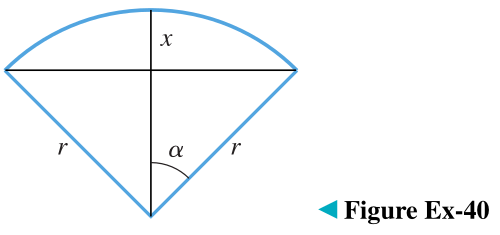
\includegraphics[width=0.5\textwidth]{../img/img_Lista2/2_40.png}
\end{figure}
\begin{enumerate}[label=(\alph*)]
\item La figura adjunta muestra un sector de radio $r$ y ángulo central $2 \alpha$. Suponiendo que el ángulo $\alpha$ es pequeño, utilice la aproximación cuadrática local de $\cos \alpha$ en $\alpha = 0$ para demostrar que $x \approx r \alpha ^2/2$. \\
La aproximación cuadrática local de $\cos \alpha$ en $\alpha = 0$ se obtiene con el polinomio de Maclaurin
\[
p_2(\alpha) = \sum_{k=0}^{2}\frac{f^{(k)} (0)}{k!} \alpha^k =  f(0) + f'(0)\alpha+ \frac{f''(0)}{2!}\alpha^2 
\] 
\begin{flushright}
(1)
\end{flushright}
\begin{center}
  \begin{tabular}{r l}
   $f(\alpha) = cos\alpha $ & $ f(0) = cos(0) = 1$ \\
   $f'(\alpha) = \frac{d}{d\alpha} cosx = -sen\alpha$ & $ f'(0) = -sen(0) = 0$ \\
   $f''(\alpha) = \frac{d^2}{d\alpha^2} cos \alpha = \frac{d}{d\alpha} -sen \alpha = -cosx$ & $ f''(0) = -cos(0) = -1$ \\
  \end{tabular}
\end{center}
Sustituyendo en (1)
\[
cos\alpha \approx 1 + 0 \alpha+ \frac{-1}{2}\alpha^2 = 1 - \frac{\alpha^2}{2} 
\]
\begin{flushright}
(2)
\end{flushright}


Observando la figura podemos concluir que $x = r - z$ (3) donde z es el cateto adyacente al triángulo rectángulo donde encontramos $\alpha$.
Bajo estos términos, $cos\alpha = \frac{z}{r} $ así que $z = cos \alpha \cdot r$.\\
Sustituyendo z  en (3) obtenemos $x = r -(cos \alpha \cdot r) $ (4).\\
Remplazando $cos\alpha$  en (4) por su aproximación antes obtenida en (2), obtenemos que 
\begin{eqnarray}
x
& = &  r -(cos \alpha \cdot r) \nonumber
\\
& \approx & r -(r \cdot (1 - \frac{\alpha^2}{2})) \nonumber
\\
& \approx  & r -(r - \frac{\alpha^2 \cdot r}{2}) \nonumber
\\
& \approx & r -r + \frac{\alpha^2 \cdot r}{2}) \nonumber
\\
& \approx & \frac{\alpha^2 \cdot r}{2} \nonumber
\end{eqnarray}
\[
\therefore x \approx \frac{r \cdot \alpha^2 }{2}
\]
\begin{flushright}
$\blacksquare$
\end{flushright}
\item Suponiendo que la Tierra es una esfera de radio $4000 mi$, use el resultado del inciso $(a)$ para aproximar la cantidad máxima en la que un arco de $100 mi$ a lo largo del ecuador divergirá de su cuerda.\\
Encontrar la cantidad en la que un arco de la Tierra divergirá del ecuador es equivalente a encontrar $x$ en el inciso anterior.
Para usar $x \approx \frac{r \cdot \alpha^2 }{2}$ conocemos que el radio es de 4000 mi pero necesitamos conocer el ángulo también. \\
Conocemos que el tamaño del arco es de 100 mi y este se puede calcular dar en términos del radio y el ángulo, siendo que:
\[
c = r \cdot \theta
\]
donde:
c es el tamaño del arco,
r es el radio,
$\theta$ es el ángulo que genera el segmento.
Despejando, podemos calcular el ángulo $\theta$:
\[
\theta = \frac{c}{r}
\]
Remplazando por los datos conocidos:
\[
\theta = \frac{100}{4000} = 0.025 rad
\]
Sin embargo, la ecuación según la figura esta dada para un ángulo $\alpha$ que es la mitad del ángulo $\theta$ que corresponde al del total del segmento.	Así que
\[
\alpha = \frac{\theta}{2} = \frac{0.025}{2}= 0.0125 rad
\]
Una vez conocidos todos los valores necesarios, podemos aplicar la fórmula para x
\begin{eqnarray}
x
& \approx &  \frac{r \cdot \alpha^2 }{2} \nonumber
\\
& \approx & \frac{4000 \cdot 0.0125^2 }{2} \nonumber
\\
& \approx  & 0.3125 ~ mi\nonumber
\\
\end{eqnarray}
$\therefore$  La cantidad máxima en la que un arco de $100 mi$ a lo largo del ecuador divergirá de su cuerda es 0.3125 mi.

\end{enumerate}


%% 6
\section{Identidad de Euler} Flores Morán Julieta Melina \\

Aplicar las definiciones de las funciones exponencial natural, seno y coseno como series de Taylor para demostrar la identidad de Euler:
\[e^{i\theta} = \cos(\theta) + i \sin(\theta)\]
y deducir, de aquí, que:
\[e^{i\pi} + 1 = 0\]

Para demostrar que $e^{i\theta} = \cos(\theta) + i \sin(\theta)$ hay que considerar las siguientes definiciones:
\[
e^x = \sum_{k=0}^{\infty}\frac{x^{k}}{k!}
\]

\[
\cos\theta = \sum_{k=0}^{\infty}\frac{(-1)^{k}}{2k!} \cdot \theta ^{2k} = 1- \frac{\theta^2}{2!} + \frac{\theta ^4}{4!} -   \frac{\theta^6}{6!} + \ldots
\]
\[
\sin\theta = \sum_{k=0}^{\infty}\frac{(-1)^{k}}{(2k+1)!} \cdot \theta ^{2k+1} =  \theta - \frac{\theta^3}{3!} + \frac{\theta ^5}{5!} -   \frac{\theta^7}{7!} + \ldots
\]
Podemos desarrollar la función de exponencial natural como serie de Taylor

\begin{eqnarray}
e^{i\theta} 
& = &   \sum_{k=0}^{\infty}\frac{(i\theta)^{k}}{k!} \nonumber
\\
& = & 1 + i\theta + \frac{(i\theta)^2}{2!} + \frac{(i\theta)^3}{3!}+ \frac{(i\theta)^4}{4!}+ \frac{(i\theta)^5}{5!} + \frac{(i\theta)^6}{6!} + \frac{(i\theta)^7}{7!}+ \ldots  \nonumber
\\
& = &  1 + i\theta - \frac{\theta^2}{2!} - \frac{i\theta^3}{3!}+ \frac{\theta^4}{4!}+ \frac{i\theta^5}{5!} - \frac{\theta^6}{6!} - \frac{i\theta^7}{7!}+ \ldots  \nonumber
\\\nonumber
\end{eqnarray}
Al agrupar los términos complejos y los reales.
\begin{eqnarray}
e^{i\theta} 
& = &  1 + i\theta - \frac{\theta^2}{2!} - \frac{i\theta^3}{3!}+ \frac{\theta^4}{4!}+ \frac{i\theta^5}{5!} - \frac{\theta^6}{6!} - \frac{i\theta^7}{7!}+ \ldots  \nonumber
\\
& = &  [1 - \frac{\theta^2}{2!} + \frac{\theta^4}{4!}- \frac{\theta^6}{6!} + \ldots ]+[i\theta   - \frac{i\theta^3}{3!}+ \frac{i\theta^5}{5!} - \frac{i\theta^7}{7!}+ \ldots]  \nonumber
\\
& = &  [1 - \frac{\theta^2}{2!} + \frac{\theta^4}{4!}- \frac{\theta^6}{6!} + \ldots ]+i[\theta   - \frac{\theta^3}{3!}+ \frac{\theta^5}{5!} - \frac{\theta^7}{7!}+ \ldots]  \nonumber
\\\nonumber
\end{eqnarray}
Estos grupos son las definiciones de $\cos\theta$ y $\sin\theta$
\begin{eqnarray}
e^{i\theta} \nonumber
& = &  [1 - \frac{\theta^2}{2!} + \frac{\theta^4}{4!}- \frac{\theta^6}{6!} + \ldots ]+i[\theta   - \frac{\theta^3}{3!}+ \frac{\theta^5}{5!} - \frac{\theta^7}{7!}+ \ldots]  \nonumber
\\
& = & \sum_{k=0}^{\infty}\frac{(-1)^{k}}{2k!} \cdot \theta ^{2k} +i [\sum_{k=0}^{\infty}\frac{(-1)^{k}}{(2k+1)!} \cdot \theta ^{2k+1}] \nonumber
\\
& = & \cos\theta +i [\sin\theta] \nonumber
\\ \nonumber
\end{eqnarray}
\[
\therefore e^{i\theta} = \cos(\theta) + i \sin(\theta)
\]
\begin{flushright}
$\blacksquare$
\end{flushright}
Con este resultado, sustituyendo $\theta$ por $\pi$ :
\begin{eqnarray}
e^{i\pi} \nonumber
& = &  \cos(\pi) + i \sin(\pi) \nonumber
\\
& = &  -1 + i (0) \nonumber
\\
& = &  -1\nonumber
\\ \nonumber
\end{eqnarray}
Considerando $e^{i\pi} = -1$, se puede deducir que 
\[
e^{i\pi} +1 = 0
\]

\subsection*{\centering \textbf{ \LARGE Tercera Parte}}


%% 11, 28, 31 y 41
%% 25, 31 y 40

%% 1 ---------------------------------------------------------------------------------------------------------------------------------------------------------------------------------------------------------------------------------
\section{Ejercicio 11} Flores Morán Julieta Melina \\

\begin{figure}[h!]
\centering
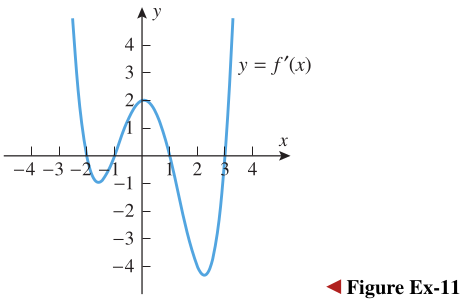
\includegraphics[width=0.6\textwidth]{../img/img_Lista2/3_11.png}
\end{figure}
La figura adjunta muestra la gráfica de $y = f'(x)$ para una función $f$ no especificada.
\begin{enumerate}[label=(\alph*)]
\item ¿Para qué valores de $x$ la curva $y = f(x)$ tiene una recta tangente horizontal?\\
  Dado que $y=f'(x)$ representa la pendiente de la recta tangente a $f(x)$, cuando $f'(x)=0$ la pendiente de la recta tangente es horizontal. Por tanto, los valores de $x$ son $-2,-1,1,3$.

\item ¿En qué intervalos la curva $y = f(x)$ tiene rectas tangentes con pendiente positiva?\\
  $(-\infty,-2),(-1,1),(3,+\infty)$.

\item ¿En qué intervalos la curva $y = f(x)$ tiene rectas tangentes con pendiente negativa?\\
  $(-2,-1), (1,3)$.

\item Dado que $g(x) = f(x) \sin x$, encuentre $g''(0)$.
  $$g'(x)=f(x)\cdot \cos x + \sin x \cdot f'(x)$$
  $$g''(x)=(-\sin xf(x) + cosxf'(x)) + (\sin xf''(x)+\cos xf'(x))$$
  \begin{equation*}
    \begin{split}
      g''(0)
      &= (-\sin 0 \cdot f(0) + cos0\cdot f'(0)) + (\sin 0\cdot f''(0)+\cos 0\cdot f'(0))\\
      &= f'(0) + f'(0) \\
      &= 2+2\\
      &=4
    \end{split}
  \end{equation*}
  
\end{enumerate}

%% 2 ---------------------------------------------------------------------------------------------------------------------------------------------------------------------------------------------------------------------------------
\section{Ejercicio 28} Flores Morán Julieta Melina \\

En cada parte, evalúa la expresión dado que $f(1)=1$, $g(1)=-2$, $f'(1)=3$ y $g'(1)=-1$.
\begin{enumerate}[label=(\alph*)]
\item $\frac{d}{dx} \lbrack f(x)g(x) \rbrack \vline _{x=1}$
  \begin{equation*}
    \begin{split}
      \frac{d}{dx} \left[ f(x)g(x) \right] \vline _{x=1}
      & = [f(x)g'(x)+g(x)f'(x)] \vline _{x=1} \\
      & = f(1)g'(1)+g(1)f'(1) \\
      & = (1 \cdot -1) + (-2 \cdot 3) \\
      & = -1 + (-6) \\
      & = -1-6 \\
      & =-7
    \end{split}
  \end{equation*}

\item $\frac{d}{dx} \lbrack \frac{f(x)}{g(x)} \rbrack \vline _{x=1}$
  \begin{equation*}
    \begin{split}
      \frac{d}{dx} \left [ \frac{f(x)}{g(x)} \right ] \vline _{x=1}
      & = \left[ \frac{g(x)f'(x)-f(x)g'(x)} {\left[ g(x) \right]^2} \right ] \vline _{x=1} \\
      & = \frac{g(1)f'(1)-f(1)g'(1)}{\lbrack g(1) \rbrack ^2}\\
      & = \frac{(-2 \cdot 3)-(1 \cdot -1)}{(-2) ^2}\\
      & = \frac{(-6)-(-1)}{4}\\
      & = \frac{-6+1}{4}\\
      & = - \frac{5}{4}\\
    \end{split}
  \end{equation*}

\item $\frac{d}{dx} \lbrack \sqrt{f(x)} \rbrack \vline _{x=1}$
  \begin{equation*}
    \begin{split}
      \frac{d}{dx} \left[ \sqrt{f(x)} \right] \vline _{x=1}
      & = \frac{d}{dx} { [f(x)]^{\frac{1}{2}} } \vline _{x=1} \\
      & = \left[ \frac{1}{2}[f(x)]^{-\frac{1}{2}} \cdot f'(x)\right] \vline _{x=1} \\
      & = \frac{1}{2}[f(1)]^{-\frac{1}{2}} \cdot f'(1)  \\
      & = \frac{1}{2}(1)^{-\frac{1}{2}} \cdot 3  \\
      & = \frac{1}{2}(1) \cdot 3  \\
      & = \frac{3}{2}
    \end{split}
  \end{equation*}

\item $\frac{d}{dx} \lbrack f(1)g'(1) \rbrack$
  \begin{equation*}
    \begin{split}
      \frac{d}{dx} \lbrack f(1)g'(1) \rbrack
      & = \frac{d}{dx} \lbrack 1 \cdot -1 \rbrack \\
      & = \frac{d}{dx} \lbrack -1 \rbrack \\
      & = 0
    \end{split}
  \end{equation*}
  
\end{enumerate}

%% 3 ---------------------------------------------------------------------------------------------------------------------------------------------------------------------------------------------------------------------------------
\section{Ejercicio 31} Flores Morán Julieta Melina\\

Encuentre $f'(x)$.
\begin{enumerate}[label=(\alph*)]
\item $f(x)=\sqrt{3x+1} (x-1)^2$ \\
  $f(x) =(3x+1)^{\frac{1}{2}}(x-1)^2$
  \begin{equation*}
    \begin{split}
      f'(x)
      &= \left[ (3x+1)^{\frac{1}{2}} \cdot \frac{d}{dx}(x-1)^2 \right]
         + \left[ (x-1)^2 \cdot \frac{d}{dx}(3x+1)^{\frac{1}{2}} \right]\\
      &= \left\lbrace (3x+1)^{\frac{1}{2}} \left[ 2(x-1)\cdot \frac{d}{dx}(x-1)\right] \right\rbrace
         + \left\lbrace (x-1)^2\left[\frac{1}{2}(3x+1)^{-\frac{1}{2}}\cdot \frac{d}{dx}(3x+1)\right] \right\rbrace\\
      &= \left\lbrace (3x+1)^{\frac{1}{2}} \left[ 2(x-1)\cdot 1\right] \right\rbrace
         + \left\lbrace (x-1)^2\left[\frac{1}{2}(3x+1)^{-\frac{1}{2}}\cdot 3\right] \right\rbrace\\
         &= 2(x-1)(3x+1)^{\frac{1}{2}} + \frac{3(x-1)^2}{2(3x+1)^{\frac{1}{2}}}\\
         &= \frac{\left\lbrace2(3x+1)^{\frac{1}{2}}\left[2(x-1)(3x+1)^{\frac{1}{2}}\right]\right\rbrace
           + 3(x-1)^2}{2(3x+1)^{\frac{1}{2}}}\\
         &= \frac{4(x-1)(3x+1) + 3(x-1)^2}{2(3x+1)^{\frac{1}{2}}}\\
         &= \frac{(x-1)\left[ 4(3x+1)+3(x-1)  \right]}{2(3x+1)^{\frac{1}{2}}}\\
         &= \frac{(x-1)\left[ 12x+4+3x-3  \right]}{2(3x+1)^{\frac{1}{2}}}\\
         &= \frac{(x-1)(15x+1)}{2(3x+1)^{\frac{1}{2}}}\\
         &= \frac{(x-1)(15x+1)}{2\sqrt{3x+1}}\\
    \end{split}
  \end{equation*}
  
\item $f(x)=\left( \frac{3x+1}{x^2} \right)^3$
  \begin{equation*}
    \begin{split}
      f'(x)
      &= 3\left( \frac{3x+1}{x^2} \right)^2 \frac{d}{dx}\left( \frac{3x+1}{x^2} \right)\\
      &= 3\left( \frac{3x+1}{x^2} \right)^2 \frac{d}{dx}\left[(3x+1)(x^{-2})\right]\\
      &= 3\left( \frac{3x+1}{x^2} \right)^2 \left[
      (3x+1)\frac{d}{dx}(x^{-2})+(x^{-2})\frac{d}{dx}(3x+1) \right]\\
      &= 3\left( \frac{3x+1}{x^2} \right)^2 \left[
      (3x+1)\frac{d}{dx}(x^{-2})+(x^{-2})\frac{d}{dx}(3x+1) \right]\\
      &= 3\left( \frac{3x+1}{x^2} \right)^2 \left[ (3x+1)(-2x^{-3})+(x^{-2})(3) \right]\\
      &= 3\cdot \frac{(3x+1)^2}{(x^2)^2} \left( -6x^{-2}-2x^{-3}+3x^{-2} \right)\\
      &= 3 \cdot \frac{(3x+1)^2}{x^4} \left( -3x^{-2}-2x^{-3} \right)\\
      &= -\frac{3(3x+1)^2}{x^4} \left( \frac{3}{x^2}+\frac{2}{x^3} \right)\\
      &= -\frac{3(3x+1)^2}{x^4} \left( \frac{3x+2}{x^3} \right)\\
      &= -\frac{3(3x+1)^2(3x+2)}{x^7} \\
    \end{split}
  \end{equation*}
  
\end{enumerate}

%% 4 ---------------------------------------------------------------------------------------------------------------------------------------------------------------------------------------------------------------------------------
\section{Ejercicio 41} Zarco Romero José Antonio \\

Supongamos que $f'(x) = 2x \cdot f(x)$ y $f(2) = 5$.
\begin{enumerate}[label=(\alph*)]
\item Encuentra $g'(\pi / 3)$ si $g(x)=f(\sec x)$.
  \begin{equation*}
    \begin{split}
      g'(x)
      &= f'(\sec x)\frac{d}{dx}\sec x\\
      &= 2\sec x\cdot f(\sec x)\frac{d}{dx}\sec x\\
      &= 2\sec x\cdot f(\sec x)\cdot \sec x\tan x\\
      g'(\frac{\pi}{3})
      &= 2\sec \frac{\pi}{3}\cdot f(\sec \frac{\pi}{3})\cdot \sec \frac{\pi}{3}\tan \frac{\pi}{3}\\
      &= 2\cdot 2 \cdot f(2)\cdot 2\cdot \sqrt{3}\\
      &= 8\cdot 5 \sqrt{3}\\
      &= 40\sqrt{3}\\
    \end{split}
  \end{equation*}
  
\item Encuentra $h'(2)$ si $h(x)=\left[ f(x)/(x-1) \right]^4$.
  \begin{equation*}
    \begin{split}
      h'(x)
      &= 4\left(\frac{f(x)}{x-1}\right)^3\frac{(x-1)f'(x)-f(x)}{(x-1)^2}\\
      &= 4\left(\frac{f(x)}{x-1}\right)^3\frac{(x-1)(2x\cdot f(x))-f(x)}{(x-1)^2}\\
      &= 4\cdot \frac{[f(x)]^3}{(x-1)^3}\cdot \frac{f(x)[(x-1)(2x)-1]}{(x-1)^2}\\
      &= \frac{4[f(x)]^3}{(x-1)^3}\cdot \frac{f(x)(2x^2-2x-1)}{(x-1)^2}\\
      &= \frac{4[f(x)]^4(2x^2-2x-1)}{(x-1)^5}\\
      h'(2)
      &= \frac{4[f(2)]^4(2(2^2)-2\cdot 2-1)}{(2-1)^5}\\
      &= \frac{4(5)^4(2(4)-4-1)}{1^5}\\
      &= 4\cdot 625\cdot 3\\
      &= 7500
    \end{split}
  \end{equation*}
\end{enumerate}

%% 5 ---------------------------------------------------------------------------------------------------------------------------------------------------------------------------------------------------------------------------------
\section{Ejercicio 25} Zarco Romero José Antonio \\

Utilice la diferenciación implícita para encontrar la pendiente de la recta tangente a la curva en el punto especificado y verifique que su respuesta sea consistente con la gráfica adjunta en la página siguiente.
\begin{equation*}
x^4+y^4=16; \qquad (1, \sqrt[4]15) \qquad \text{\textbf{[Lamé’s special quartic]}}
\end{equation*}
\begin{figure}[H]
\centering
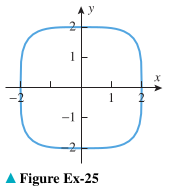
\includegraphics[width=0.35\textwidth]{../img/img_Lista2/3_25.png}
\end{figure}
Derivamos y con respecto de x
\begin{align*}
  4x^3+4y^3\frac{dy}{dx}=0\\
  4(x^3+y^3\frac{dy}{dx})=0\\
  x^3+y^3\frac{dy}{dx}=0\\
  \therefore \frac{dy}{dx}=-\frac{x^3}{y^3}
\end{align*}
Evaluamos en el punto $(1, \sqrt[4]15)$
\begin{equation*}
  \begin{split}
    \frac{dy}{dx}
    &=-\frac{x^3}{y^3} ~ \vline_{(1, \sqrt[4]15)}\\
    &= -\frac{1^3}{(\sqrt[4]15)^3}\\
    &= -\frac{1}{\sqrt[4]{15^3}}\\
    &\approx -0.1312\\
  \end{split}
\end{equation*}

%% 6 ---------------------------------------------------------------------------------------------------------------------------------------------------------------------------------------------------------------------------------
\section{Ejercicio 31} Zarco Romero José Antonio \\

Utilice la diferenciación implícita para encontrar la derivada especificada.
\[ a^2 \omega^2 + b^2 \lambda^2 = 1 \text{ ($a$, $b$ constantes);}\qquad d\omega /d\lambda \]

Diferenciando implícitamente ambos lados de la ecuación con respecto a $\lambda$ produce
\begin{align*}
  2a^2\omega \frac{d\omega}{d\lambda}+2b^2\lambda=0\\
  2(a^2\omega \frac{d\omega}{d\lambda}+b^2\lambda)=0\\
  a^2\omega \frac{d\omega}{d\lambda}+b^2\lambda=0\\
  a^2\omega \frac{d\omega}{d\lambda}=-b^2\lambda\\
  \therefore \frac{d\omega}{d\lambda}=-\frac{b^2\lambda}{a^2\omega}\\
\end{align*}

%% 7 ---------------------------------------------------------------------------------------------------------------------------------------------------------------------------------------------------------------------------------
\section{Ejercicio 40} Zarco Romero José Antonio \\

Se dice que dos curvas son \textbf{ortogonales} si sus rectas tangentes son perpendiculares en cada punto de intersección, y se dice que dos familias de curvas son \textbf{trayectorias ortogonales} entre sí si cada miembro de una familia es ortogonal a cada miembro de la otra familia. Esta terminología se utiliza en estos ejercicios.

La figura adjunta muestra algunos miembros típicos de las familias de hipérbolas $xy=c$ (curvas negras) y $x^2-y^2=k$ (curvas grises), donde $c \neq 0$ y $k \neq 0$. Utilice la sugerencia del ejercicio 39 para demostrar que estas familias son trayectorias ortogonales entre sí. [\textit{Sugerencia}: para que las rectas tangentes sean perpendiculares en un punto de intersección, las pendientes de esas rectas tangentes deben ser recíprocas negativas entre sí.]
\begin{figure}[H]
\centering
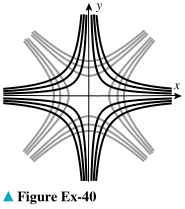
\includegraphics[width=0.35\textwidth]{../img/img_Lista2/3_40.png}
\end{figure}
Diferenciar implícitamente ambos lados de las siguientes ecuaciones con respecto a $x$ produce
\begin{enumerate}
\item $xy=c$
  \[ x\frac{dy}{dx}+1\cdot y=0 \]
  De la que obtenemos
  \begin{equation} \label{eqn: d_c_negras}
    \frac{dy}{dx}=-\frac{y}{x}
  \end{equation}
\item $x^2-y^2=k$
  \begin{align*} 
    2x - 2y\frac{dy}{dx}=0\\
    2(x-y\frac{dy}{dx})=0\\
    x-y\frac{dy}{dx}=0\\
  \end{align*}
  De la que obtenemos
  \begin{equation} \label{eqn: d_c_grises}
    \frac{dy}{dx}=\frac{x}{y}
  \end{equation}
\end{enumerate}
Al multiplicar las pendientes de las rectas tangentes de las familias de las hipérbolas, obtenemos\\
\[
  m_1 \cdot m_2 = -\frac{y}{x}\cdot \frac{x}{y}=-1\\
  \]
Por tanto, las pendientes de las rectas tangentes son recíprocas negativas entre sí, es decir:
  \[\therefore xy=c \perp x^2-y^2=k\]
Lo demostrado anteriormente aplica para cualquier valor dado de $x$ y $y$. No obstante, desarrollaremos los polinomios de las ecuaciones para encontrar los puntos de intersección de las curvas.\\
Sea $xy=c$, obtenemos que
\begin{equation} \label{eqn: y_c_negras}
y=\frac{c}{x}
\end{equation}
Sustituyendo el valor de $y$ de la ecuación \eqref{eqn: y_c_negras}
\begin{align*} 
  x^2-y^2=k \underset{y=\frac{c}{x}}{\Longrightarrow} x^2- \left( \frac{c}{x} \right) ^2=k\\
  x^2-\frac{c^2}{x^2}-k=0\\
  x^4-kx^2-c^2=0
\end{align*}
Por lo tanto, los valores de $x$ son
\begin{align*}
  x_0=\sqrt{\frac{2k+2\sqrt{k^2+4c^2}}{2}}\\
  x_1=-\sqrt{\frac{2k+2\sqrt{k^2+4c^2}}{2}}\\
  x_2=\sqrt{\frac{2k-2\sqrt{k^2+4c^2}}{2}}\\
  x_3=-\sqrt{\frac{2k-2\sqrt{k^2+4c^2}}{2}}\\
\end{align*}
Sustituyendo el valor de cada $x$ en la ecuación \eqref{eqn: y_c_negras}, obtenemos los valores de y para cada valor de $x$
\begin{align*}
  y_0=\frac{c}{\sqrt{\frac{2k+2\sqrt{k^2+4c^2}}{2}}}\\
  y_1=-\frac{c}{\sqrt{\frac{2k+2\sqrt{k^2+4c^2}}{2}}}\\
  y_2=\frac{c}{\sqrt{\frac{2k-2\sqrt{k^2+4c^2}}{2}}}\\
  y_3=-\frac{c}{\sqrt{\frac{2k-2\sqrt{k^2+4c^2}}{2}}}\\
\end{align*}
Ahora, evaluamos cada punto de intersección en la derivada de la ecuación $xy=c$
\begin{equation*}
  \begin{split}
    \frac{dy}{dx}
    &= -\frac{y}{x} ~ \vline _{(x_0,y_o)}\\
    &= - \frac{  \frac{c}{\sqrt{\frac{2k+2\sqrt{k^2+4c^2}}{2}}}}{ \sqrt{\frac{2k+2\sqrt{k^2+4c^2}}{2}}}
    &= -\frac{c}{ \frac{2k+2\sqrt{k^2+4c^2}}{2} }\\   
  \end{split}
\end{equation*}
\begin{equation*}
  \begin{split}
    \frac{dy}{dx}
    &= -\frac{y}{x} ~ \vline _{(x_1,y_1)}\\
    &=  -\frac{y}{x} ~ \vline _{\left(-\sqrt{\frac{2k+2\sqrt{k^2+4c^2}}{2}}, -\frac{c}{\sqrt{\frac{2k+2\sqrt{k^2+4c^2}}{2}}\right)}}\\
    &= - \frac { \frac{c}{\sqrt{ \frac {2k+2\sqrt{k^2+4c^2}} {2}}}}{  \sqrt{\frac{2k+2\sqrt{k^2+4c^2}}{2}}    }
    &= - \frac {c}{ \frac {2k+2\sqrt{k^2+4c^2}} {2}}
  \end{split}
\end{equation*}
\begin{equation*}
  \begin{split}
    \frac{dy}{dx}
    &= -\frac{y}{x} ~ \vline _{(x_2,y_2)}\\
    &=  -\frac{y}{x} ~ \vline _{\left(\sqrt{\frac{2k-2\sqrt{k^2+4c^2}}{2}}, \frac{c}{\sqrt{\frac{2k-2\sqrt{k^2+4c^2}}{2}}}\right)}\\
    &=  - \frac { \frac{c}{\sqrt{ \frac {2k-2\sqrt{k^2+4c^2}} {2}}}}{  \sqrt{\frac{2k-2\sqrt{k^2+4c^2}}{2}}    }
    &=  - \frac {c}{ \frac {2k-2\sqrt{k^2+4c^2}} {2}}\\
  \end{split}
\end{equation*}
\begin{equation*}
  \begin{split}
    \frac{dy}{dx}
    &= -\frac{y}{x} ~ \vline _{(x_3,y_3)}\\
    &=  -\frac{y}{x} ~ \vline _{\left(-\sqrt{\frac{2k-2\sqrt{k^2+4c^2}}{2}}, -\frac{c}{\sqrt{\frac{2k-2\sqrt{k^2+4c^2}}{2}}}\right)}\\
    &=  - \frac { \frac{c}{\sqrt{ \frac {2k-2\sqrt{k^2+4c^2}} {2}}}}{  \sqrt{\frac{2k-2\sqrt{k^2+4c^2}}{2}}    }
    &=  - \frac {c}{ \frac {2k-2\sqrt{k^2+4c^2}} {2}}\\
  \end{split}
\end{equation*}
Enseguida, evaluamos cada punto de intersección en la derivada de la ecuación $x^2-y^2=k$
\begin{equation*}
  \begin{split}
    \frac{dy}{dx}
    &= \frac{x}{y} ~ \vline _{(x_0,y_o)}\\
    &= \frac{x}{y} ~ \vline _{\left(\sqrt{\frac{2k+2\sqrt{k^2+4c^2}}{2}}, \frac{c}{\sqrt{\frac{2k+2\sqrt{k^2+4c^2}}{2}}\right)}}\\
    &= \frac{\sqrt{\frac{2k+2\sqrt{k^2+4c^2}}{2}}}{\frac{c}{\sqrt{\frac{2k+2\sqrt{k^2+4c^2}}{2}}}}\\
    &= \frac {  \frac {2k+2\sqrt{k^2+4c^2}}  {2}  } {c}\\
  \end{split}
\end{equation*}
\begin{equation*}
  \begin{split}
    \frac{dy}{dx}
    &= \frac{x}{y} ~ \vline _{(x_1,y_1)}\\
    &= \frac{x}{y} ~ \vline _{\left(-\sqrt{\frac{2k+2\sqrt{k^2+4c^2}}{2}}, -\frac{c}{\sqrt{\frac{2k+2\sqrt{k^2+4c^2}}{2}}}\right)}\\
    &= \frac{\sqrt{\frac{2k+2\sqrt{k^2+4c^2}}{2}}}{\frac{c}{\sqrt{\frac{2k+2\sqrt{k^2+4c^2}}{2}}}}\\
    &= \frac {  \frac {2k+2\sqrt{k^2+4c^2}}  {2}  } {c}\\
  \end{split}
\end{equation*}

\begin{equation*}
  \begin{split}
    \frac{dy}{dx}
    &= \frac{x}{y} ~ \vline _{(x_2,y_2)}\\
    &= \frac{x}{y} ~ \vline _{\left(\sqrt{\frac{2k-2\sqrt{k^2+4c^2}}{2}}, \frac{c}{\sqrt{\frac{2k-2\sqrt{k^2+4c^2}}{2}}}\right)}\\
    &= \frac{\sqrt{\frac{2k-2\sqrt{k^2+4c^2}}{2}}}{\frac{c}{\sqrt{\frac{2k-2\sqrt{k^2+4c^2}}{2}}}}\\
    &= \frac {  \frac {2k-2\sqrt{k^2+4c^2}}  {2}  } {c}\\
  \end{split}
\end{equation*}
\begin{equation*}
  \begin{split}
    \frac{dy}{dx}
    &= \frac{x}{y} ~ \vline _{(x_3, y_3)}\\
    &= \frac{x}{y} ~ \vline _{\left(-\sqrt{\frac{2k-2\sqrt{k^2+4c^2}}{2}}, -\frac{c}{\sqrt{\frac{2k-2\sqrt{k^2+4c^2}}{2}}}\right)}\\
    &= \frac{\sqrt{\frac{2k-2\sqrt{k^2+4c^2}}{2}}}{\frac{c}{\sqrt{\frac{2k-2\sqrt{k^2+4c^2}}{2}}}}\\
    &= \frac {  \frac {2k-2\sqrt{k^2+4c^2}}  {2}  } {c}\\
  \end{split}
\end{equation*}
Al multiplicar pendientes:\\
(x_0, y_0) : ~ ~
\[
  m_1 \cdot m_2 = -\frac{c}{ \frac{2k+2\sqrt{k^2+4c^2}}{2} }    \cdot  \frac {  \frac {2k+2\sqrt{k^2+4c^2}}  {2}  }{ c} = -1
 \] \\
(x_1, y_1) : ~ ~
\[
  m_1 \cdot m_2 = - \frac {c}{ \frac {2k+2\sqrt{k^2+4c^2}} {2}} \cdot \frac {  \frac {2k+2\sqrt{k^2+4c^2}}  {2}  } {c} =- 1
\]\\
(x_2, y_2):~ ~
\[
  m_1 \cdot m_2 = -\frac {c}{ \frac {2k-2\sqrt{k^2+4c^2}} {2}} \cdot \frac {  \frac {2k-2\sqrt{k^2+4c^2}}  {2}  } {c} = -1
  \]\\ 
(x_3, y_3): ~ ~
\[
  m_1 \cdot m_2 =  - \frac {c}{ \frac {2k-2\sqrt{k^2+4c^2}} {2}} \cdot   \frac {  \frac {2k-2\sqrt{k^2+4c^2}}  {2}  } {c} = -1
  \] \\ \\
Lo que demuestra que son recíprocas negativas entre sí y por tanto, trayectorias ortogonales.
\begin{flushright}
$\blacksquare$
\end{flushright}
\end{document}
